\graphicspath{{figures/static/}}
\chapter{输电塔结构在龙卷风作用下的静态响应分析}\label{chapter:static}

\section{引言}
大跨越输电塔结构是重要的生命线电力工程设施,具有数量大、分布广等特点,容易遭受龙
卷风的袭击,其破坏将导致供电系统的瘫痪甚至引发火灾等严重后果,造成重大经济损失。
美国输电塔设计规范已考虑龙卷风等极端天气荷载,我国输电线路设计规范尚未涉及。
为保障龙卷风多发地区电网运行安全,进行输电线路龙卷风风荷载及抗风研究具有重要的理
论和实用价值。

国内外文献研究龙卷风作用下输电塔结构响应的基本思路为:
采用Rankine或Wen模型模拟龙卷风解析风场,或采用CFD技术模拟龙卷风数值风场;
然后利用规范中风荷载计算公式将风速场转化为风荷载并施加到输电塔有限元模型上,计算
结构响应。
这一研究思路采用普通风作用下的结构参数(如体型系数等)计算龙卷风荷载,但两种风场
结构差别较大,有必要研究直接模拟输电塔结构所受龙卷风荷载的方法。

本章利用单向流固耦合方法(下文简称FSI)直接在足尺龙卷风风场中建立输电塔的刚性模
型,进行CFD计算得到结构表面受到的龙卷风风压。
结构有限元计算采用梁单元模拟输电塔结构,故本文提出将CFD计算得到的结构表面风压转
化为梁单元节点集中力的方法。
文中还介绍了利用规范方法计算龙卷风荷载并施加到输电塔结构的方法。
最后改变龙卷风的袭击角度,分别在0度、45度和90度工况下进行龙卷风荷载的计算和施加,
比较两种方法计算得到的结构轴向力和位移响应。


\section{\SI{500}{kV}南京三江口长江大跨越工程介绍}
\SI{500}{kV}南京三江口长江大跨越工程是山西阳城电厂二期工程电力送出江苏省
内配套等输变电工程的重要组成部分,跨越点在长江南京河段的三江口节点位置。
按耐—直—直—耐实施跨越,档距分布为\SI{520}{m}-\SI{1770}{m}-\SI{520}{m}(图\ref{fig:tower-line}),跨越塔与跨越塔之间的输电线矢高为\SI{132.4}{m},跨越塔与锚塔之间的输电线矢高为\SI{50}{m}。
\begin{figure}[!htbp]
	\centering
	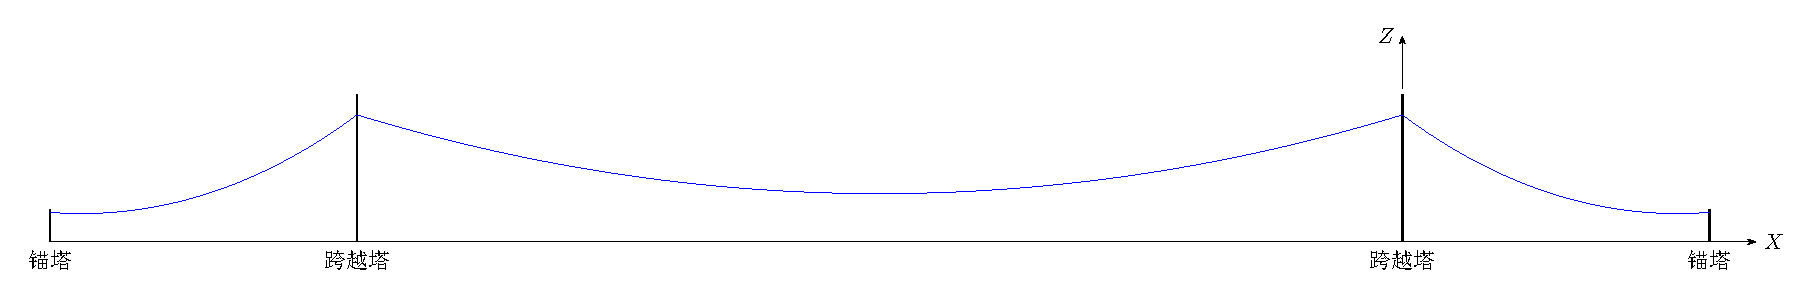
\includegraphics[width=\textwidth]{tower_line_system.pdf}
	\caption{三江口大跨越示意图}
	\label{fig:tower-line}
\end{figure}

大跨越南、北跨越塔均为双回路蝶型布置的钢管塔,呼高\SI{215}{m},全高\SI{249.5}{m},根开\SI{49.6}{m},单基塔重(含旋梯及走道)共\SI{1924}{t}。
钢管塔最大管径\SI{1480}{mm},相应壁厚\SI{25}{mm},钢管材质采用Q345B和Q235B级钢,最大螺栓直径\SI{56}{mm},螺栓采用6.8级和8.8级两种。
大跨越输电塔(下文简称大跨越塔)实物如图\ref{fig:real-tower}所示。
锚塔为单回干字型角钢塔,锚塔横担垂直于跨越段中心线布置,根开为\SI{16}{m}$\times$\SI{24}{m}布置,呼高\SI{24}{m},全高\SI{55}{m},单基塔重\SI{106}{t}。
每个回路分别对应2基铁塔,共使用4基锚塔。

导线采用四分裂布置,型号为 AACSR/EST-500 特强钢芯铝合金绞线,两根地线采用 36芯的OPGW-325型复合光缆,光缆为层绞结构。
导线、OPGW均为整根,跨越耐张段没有接头。锚塔上跳线采用LGJ-630/45型钢芯铝绞线,越侧耐张绝缘子串引流线夹与LGJ-630/45型钢芯铝绞线匹配。跨越塔导线采用四联530k N级盘瓷悬垂绝缘子串,OPGW采用双联预绞式悬垂金具串;锚塔导线采用六联400k N级盘瓷耐张绝缘子串,OPGW采用预绞式耐张金具串。
\begin{figure}[!htbp]
	\centering
	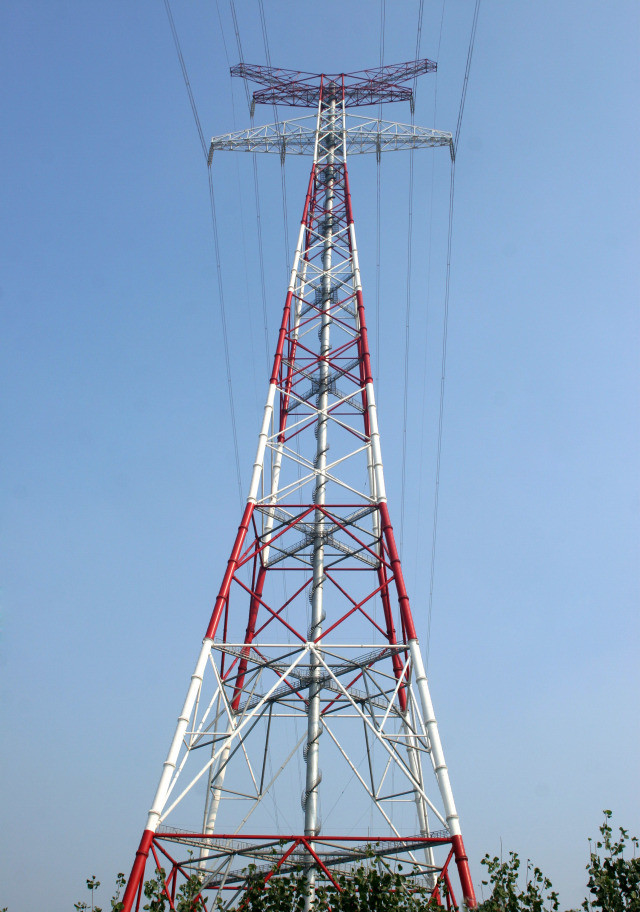
\includegraphics[width=\textwidth]{tower.png}
	\caption{三江口大跨越输电塔}
	\label{fig:real-tower}
\end{figure}

\subsection{输电塔有限元模型}\label{sec:tower-fea}
本文选择大型通用有限元软件ANSYS Mechanical APDL进行输电塔建模。

选用二节点非线性三维梁单元BEAM 188模拟输电塔构件。
单元每个节点处包括三个平动自由度和三个转动自由度。
输电塔构件之间为多孔螺栓连接,有限元模型以刚性节点模拟。
输电塔的有限元模型见\ref{fig:tower-fea}所示。
考虑到输电塔为空间对称结构,取塔的底面中心为坐标原点,高度方向为$Z$轴方向,输电线方向为$X$轴方向(图\ref{fig:tower-line}、\ref{fig:tower-fea})。
\begin{figure}[!htbp]
	\centering
	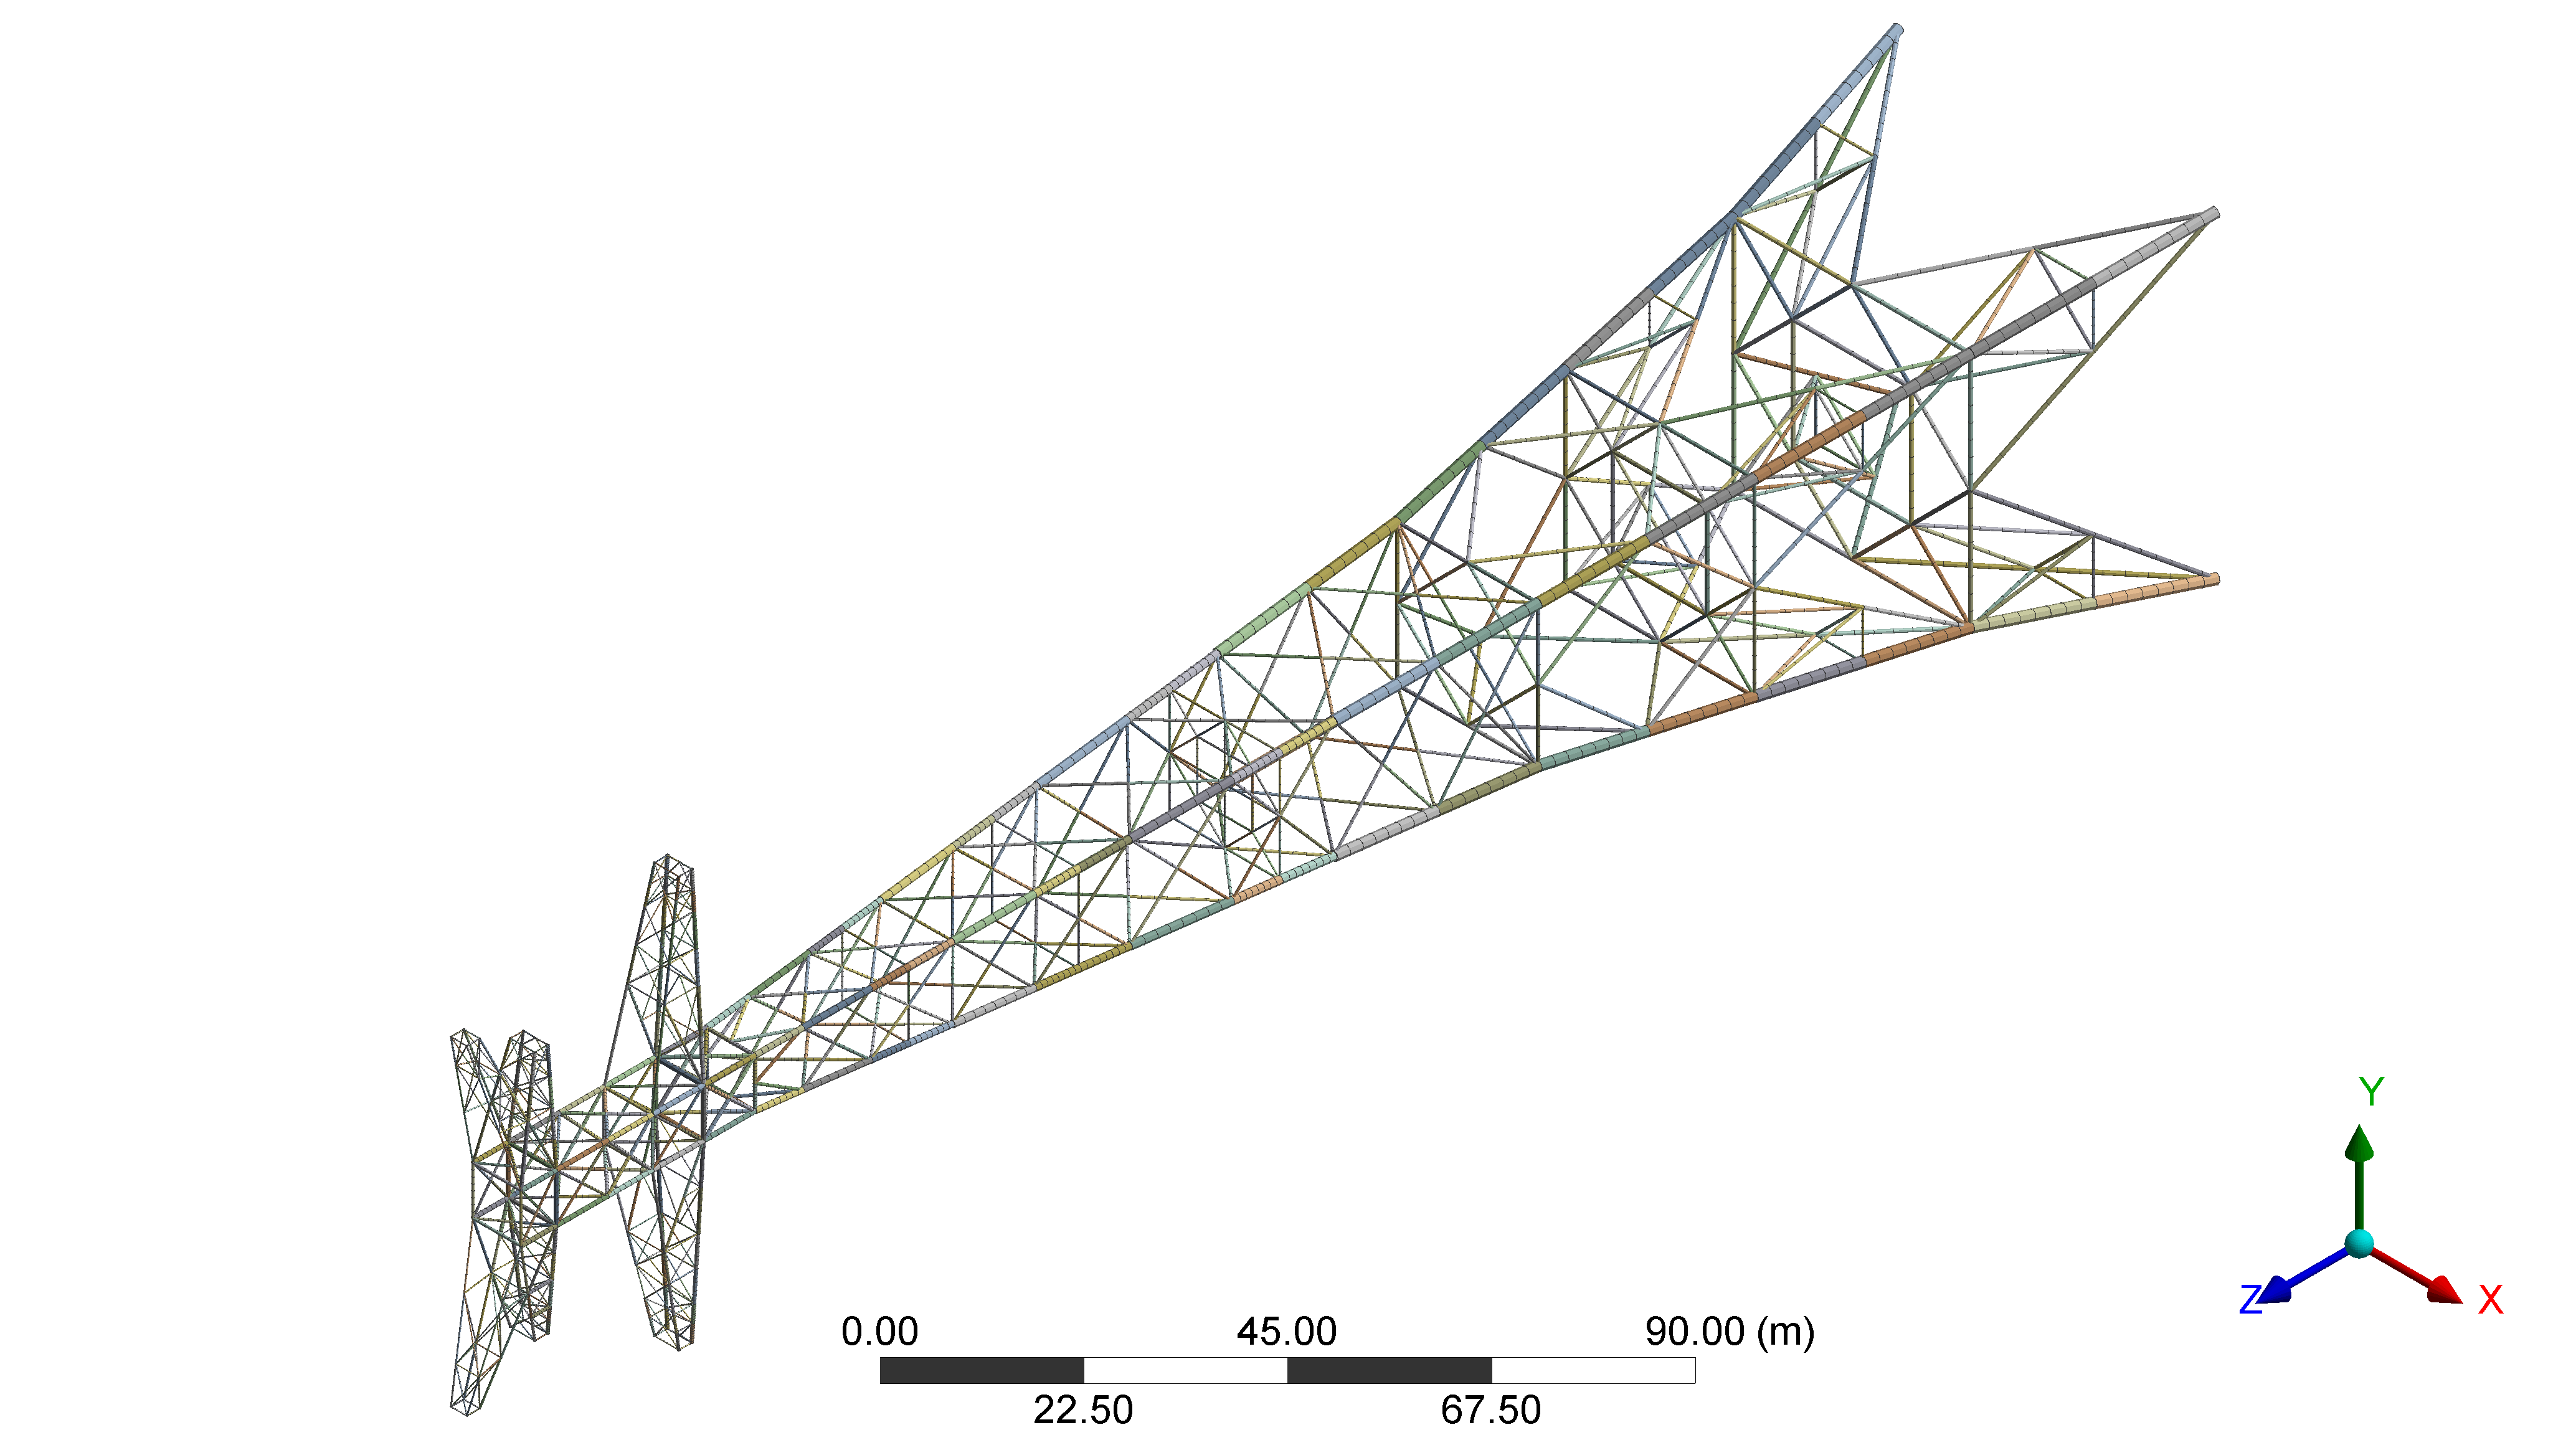
\includegraphics[width=\textwidth]{tower_fea.png}
	\caption{输电塔有限元模型}
	\label{fig:tower-fea}
\end{figure}


\subsection{输电塔结构模态分析}
本节对大跨越输电塔结构进行模态分析,计算其固有频率及振型,与文献对比,以验证输电塔有限元模型的正确性,并为后续的动态响应分析提供参考。

输电塔各阶固有频率及其与文献\cite{ren2010tower}的对比见表\ref{tab:freq},
各阶振型见图\ref{fig:modes}所示。

\begin{table}[!htbp]
	\centering
	\caption{输电塔固有频率$/\SI{}{Hz}$}
	\label{tab:freq}
	\begin{tabu} to 1.0\textwidth {X[1.5,c] X[1,c] X[1,c] X[1,c] X[1,c] X[1,c] X[1,c] X[1,c] X[1,c] X[1,c]}
		\toprule
		振型                    & 1     & 2     & 3     & 4     & 5     & 6     & 7     & 8     & 9     \\
		\midrule
		频率\cite{ren2010tower} & 0.609 & 0.612 & 1.102 & 1.558 & 1.608 & 2.113 & 2.296 & 2.407 & 3.046 \\
		频率                    & 0.613 & 0.615 & 1.093 & 1.565 & 1.594 & 2.084 & 2.312 & 2.363 & 2.368 \\
		\bottomrule
	\end{tabu}
\end{table}

\begin{figure}[!htbp]
	\centering
	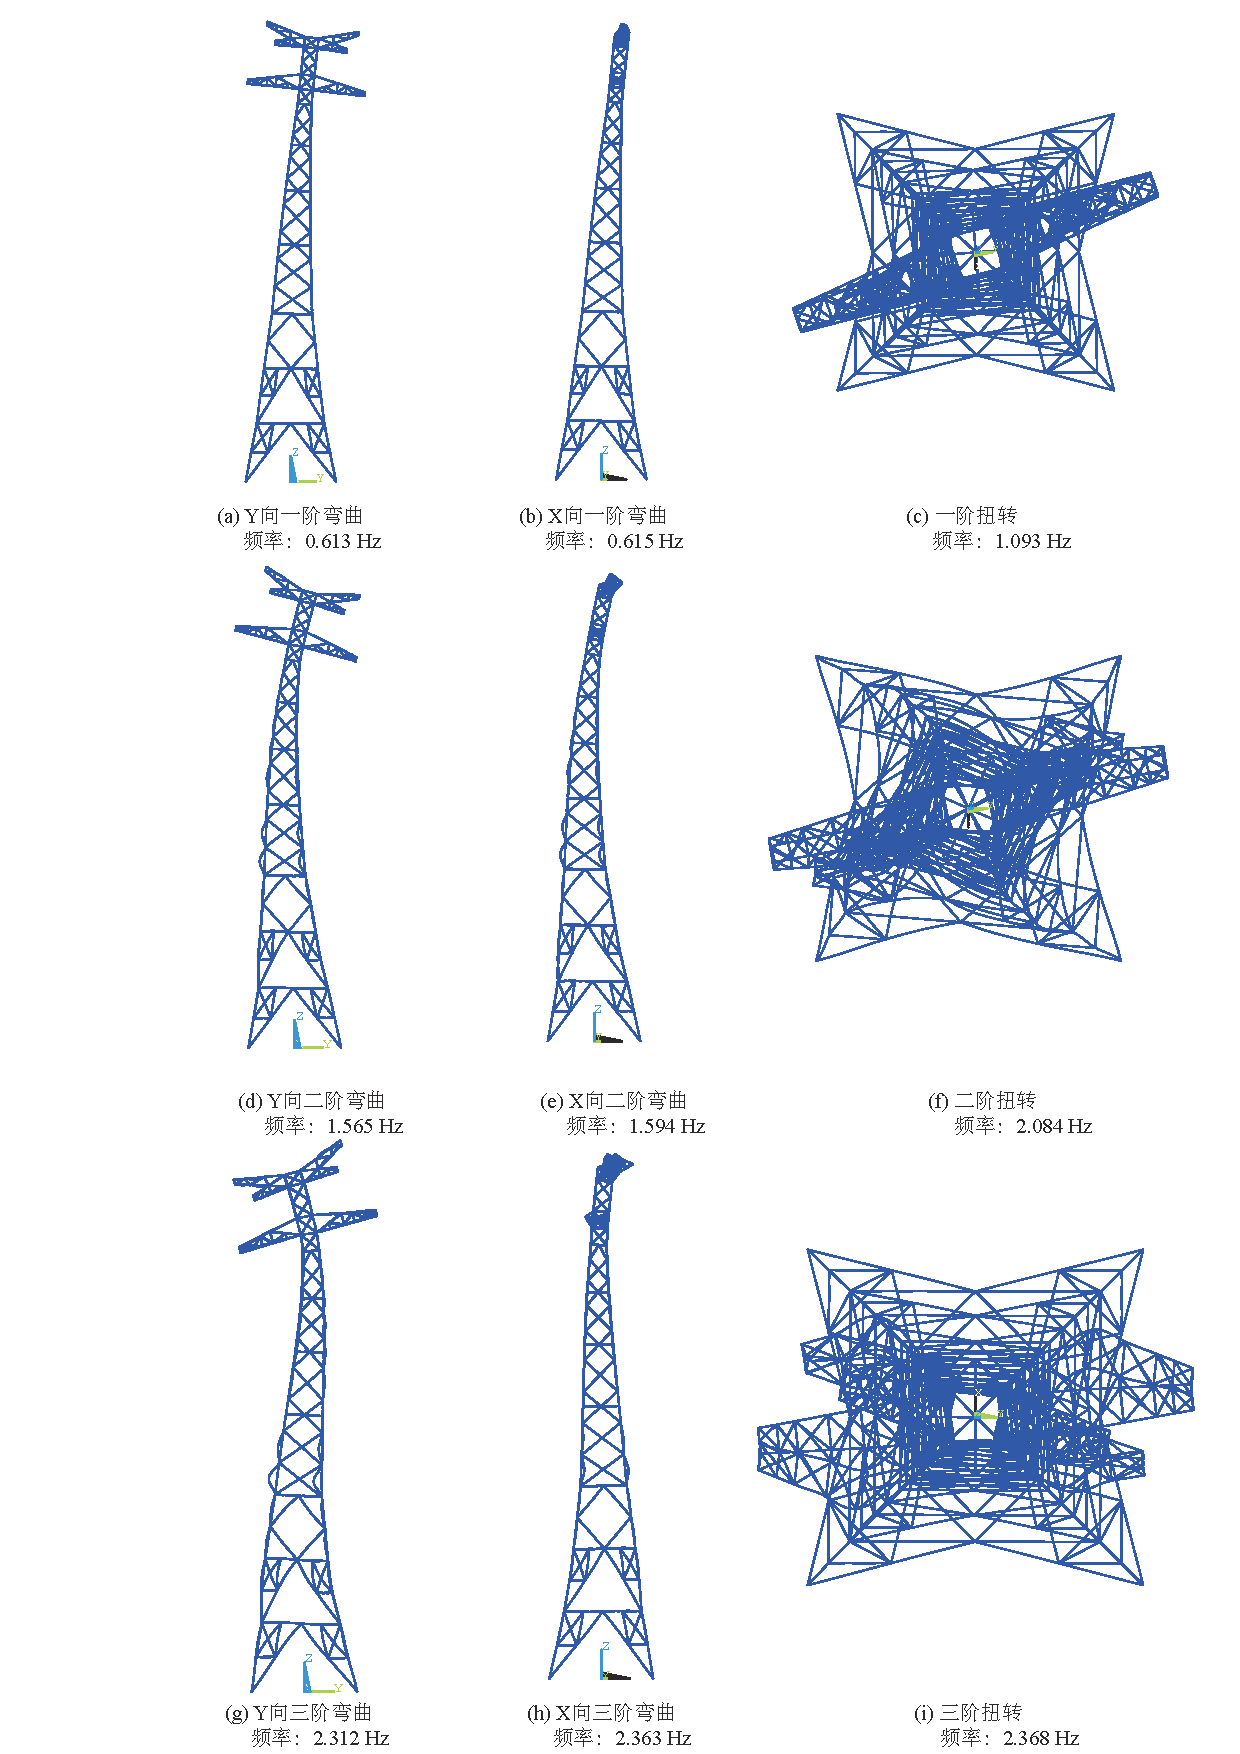
\includegraphics[width=0.9\textwidth]{modes.pdf}
	\caption{输电塔各阶振型图}
	\label{fig:modes}
\end{figure}

本章主要进行输电塔结构在龙卷风作用下的静态响应分析,即忽略龙卷风的平移效应,选定龙卷风核心相应于输电塔结构中心的位置,进行静力弹塑性分析。输电塔结构受到的主要荷载为:
\begin{enumerate}
	\item 重力荷载
	\item 输电塔受到的龙卷风涡旋风场的荷载
	\item 输电线传到输电塔的荷载
\end{enumerate}
其中忽略了龙卷风对输电线的荷载,主要是因为:
\begin{enumerate}
	\item 龙卷风路径宽度较小,F1-F2级龙卷风的路径宽度为\SI{60}{m}-\SI{150}{m}。
	\item 输电线受到的风荷载作用机制比较复杂。
\end{enumerate}

\section{输电塔龙卷风荷载计算的FSI方法}

\subsection{单向流固耦合方法介绍}

\subsection{包含输电塔刚性模型的龙卷风风场}\label{sec:tornado-fsi}
输电塔结构可分为梁柱主体框架和支撑体系,将输电塔整体的刚性模型包含进风场时,发现划分的网格数量巨大,需要较长时间才能完成CFD计算。
故本文采用的方法如下:首先在SolidWorks中用实体建立输电塔结构主体梁柱框架模型,忽略迎风效应(截面)较小的支撑等构件,然后从代表足尺龙卷风风场的圆柱体中利用布尔运算减去输电塔梁柱实体,生成包含输电塔刚性模型的计算流域。支撑等构件受到的风荷载的计算方法在第2.4\todo{Change this ref.}节中介绍。

在该计算流域上设置第\ref{sec:full-tornado}足尺龙卷风风场的边界条件,
并将输电塔刚性模型表面的边界条件设置为不可滑移壁面。
利用ICEM CFD软件进行网格划分,先采用Octree算法将计算流域初步划分为六面体和四面体混合的非结构化网格,再将生成的网格以Delaunay算法进行优化。
网格划分过程采用以下选项提高网格质量:控制输电塔表面网格划分的最大单元尺寸为0.4 m;
同时在输电塔表面设置厚度为1.0 m的棱柱形单元膨胀层网格(Prism Layers);
并以输电塔中心建立半径为150 m的球状区域,在此区域内进行网格加密以尽可能精确离散结构表面。
计算流域底部和输电塔刚性模型表面的网格划分见图\ref{fig:mesh}所示。

考虑到龙卷风风场压强分布的梯度较大,故CFD计算采用PISO求解方法,压强离散采用PRESTO!格式\cite{fluent2015user}。

\begin{figure}[!htpb]
	\centering
	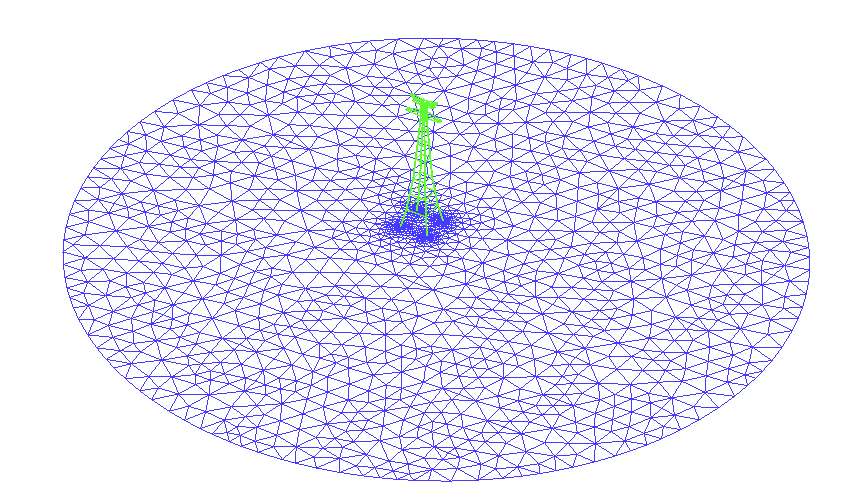
\includegraphics[width=0.6\textwidth]{mesh.png}
	\caption{输电塔周围计算流域网格}
	\label{fig:mesh}
\end{figure}

设置输电塔结构表面的压强积分值为求解监测值,迭代过程中当残差和压强积分检测值趋于稳定时结束计算。
\SI{20}{m}高度处流场剖面速度矢量分布和结构表面风压云图分别见图\ref{fig:velocity}和图\ref{fig:pressure}所示。
后处理提取输电塔梁柱表面受到的风压,格式为风压点坐标及风压值,见表。

\begin{figure}[!htpb]
	\centering
	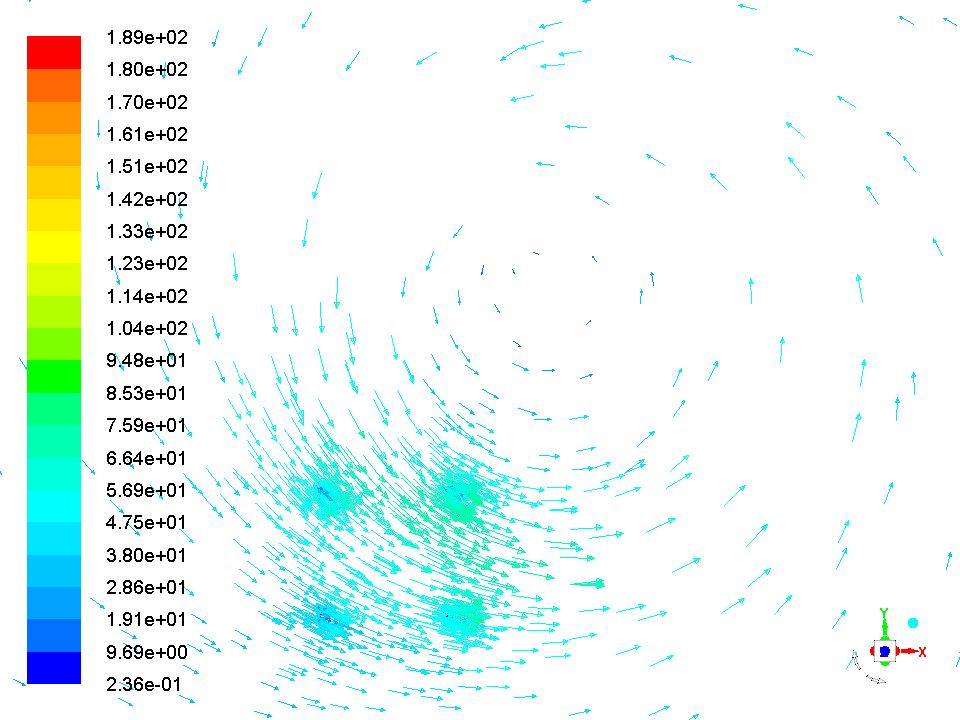
\includegraphics[width=1.0\textwidth]{velo.jpg}
	\caption{\SI{20}{m}高度处风速矢量图}
	\label{fig:velocity}
\end{figure}

\begin{figure}[!htpb]
	\centering
	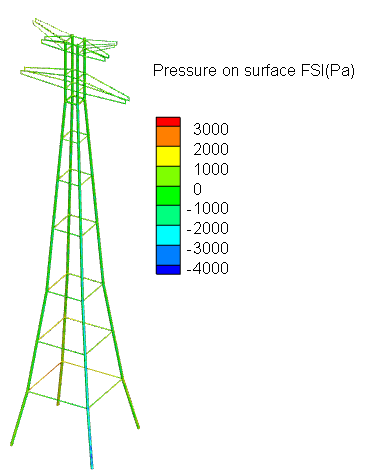
\includegraphics[width=0.4\textwidth]{pres.png}
	\caption{输电塔表面风压}
	\label{fig:pressure}
\end{figure}

\begin{table}[!htbp]
	\caption{输电塔表面CFD风压输出}
	\label{tab:pressure}
	\centering
	\begin{tabu} to 1.0\textwidth {X[c] X[c] X[c] X[1.5,c]}
		\toprule
		$X(\mathrm{m})$ & $Y(\mathrm{m})$ & $Z(\mathrm{m})$ & Pressure$(\mathrm{Pa})$ \\
		\midrule
		-94.756         & -95.510         & 0.000           & 1.906E+03               \\
		-45.910         & -94.756         & 0.000           & -1.664E+03              \\
		$\vdots$        & $\vdots$        & $\vdots$        & $\vdots$                \\
		-69.484         & -95.910         & 249.707         & 8.067E+02               \\
		\bottomrule
	\end{tabu}
\end{table}

\subsection{龙卷风风压转化为输电塔梁单元节点集中力}
在ANSYS Mechanical APDL中采用梁单元模拟输电塔结构,这就带来了CFD计算得到的龙卷风风压如何施加到梁单元上的问题。设计如下算法以实现风压转化为梁单元节点集中力。
由于流场网格对刚性输电塔表面的离散,使得风压点的位置与实际的输电塔结构表面存在偏差。
因此需要设计算法实现如下功能:

\begin{figure}[!htbp]
	\centering
	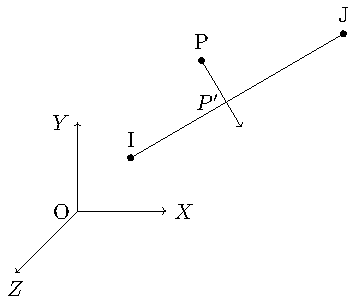
\includegraphics[width=0.6\textwidth]{algo.pdf}
	\caption{CFD风压点$P$与梁单元$IJ$示意图}
	\label{fig:algo}
\end{figure}

\begin{itemize}
	\item 判别每个CFD风压点作用于哪个有限元梁单元。
	\item 将单个CFD风压点的风压(垂直于该风压点作用的梁单元的表面)分解到整体坐标系中。
	\item 将单个有限元梁单元所受所有CFD风压点的压力进行合成,并分配到该单元节点上。
\end{itemize}

任意CFD风压点$P$与某个梁单元$IJ$示意图见图\ref{fig:algo},图中点$P'$为风压点$P$在梁单元轴线$IJ$上的投影。
由于本文研究的输电塔为钢管塔,即梁$IJ$的表面为柱面,设其外径为$R_{IJ}$,则$PP'$即为风压作用于梁$IJ$的方向。
首先通过如下准则判断风压点$P$是否作用于梁单元$IJ$上:
\begin{itemize}
	\item $P'$是否在线$IJ$内部?
	\item $PP'$是否近似等于单元$IJ$外径?
\end{itemize}
当同时满足这两个条件时,认为风压点$P$作用于梁单元$IJ$上,数学表达见式\eqref{eqn:cri}。
\begin{gather}\label{eqn:cri}
	\bm{P'I}\cdot\bm{P'J} < 0  \nonumber \\
	|PP'-R_{IJ}| < \epsilon
\end{gather}
式中点$P'$的坐标可由式\eqref{eqn:op}计算,
\begin{equation}\label{eqn:op}
	\bm{OP'}=\bm{OI} - \left( \frac{\bm{PI}\cdot\bm{IJ}}{|IJ|^2} \right)\bm{IJ}
\end{equation}
风压点$P$作用于梁单元$IJ$上的风压在整体坐标系下的分量为
\begin{equation}
	(p_X, p_Y, p_z) = p\frac{\bm{PP'}}{|PP'|}
\end{equation}

根据上述判别法则,对每个CFD风压点与每根梁单元进行判别,可确定每根梁单元所受的所有CFD风压点及各自的风压分量。
下面介绍将单个有限元梁单元所受所有CFD风压点的压力进行合成,并分配到该单元节点上的方法。
\begin{enumerate}
	\item 计算单个有限元梁单元$IJ$受到的所有风压点处风压分量的平均$\bar{p_X},\bar{p_Y},\bar{p_Z}$;
	\item 将风压根据梁表面面积转化为合力$F_X=2\pi R_{IJ} |IJ| \bar{p_X}$,$Y,Z$方向类似;
	\item 将风压合力分量平分到梁单元$I$、$J$节点上。
\end{enumerate}
至此,完成了将CFD风压传递给有限元梁单元节点荷载的算法。

\subsubsection{测试算例}
设计如图\ref{fig:example}所示的算例测试该算法的有效性。
悬臂钢管柱外径$R=\SI{1.0}{m}$,高度$H=\SI{9}{m}$,单侧受到径向压强,分布为$p_r(y)=p_0\frac{y}{H},p_0=\SI{100}{Pa}$。
据此编程生成风压点及相应的压强值,作为本文算法的输入,输出各节点施加的集中力见表\ref{tab:example-force}所示。
计算各节点集中力的合力见表\ref{tab:example-force},与理论合力$F_X = \int_{0}^{H}\int_{\pi/2}^{3\pi/2}p_r(y)\cos(\theta+\pi)R \mathrm{d} \theta \mathrm{d} y = p_0 RH=\SI{900}{Pa}$误差很小。

\begin{figure}[!htbp]
	\centering
	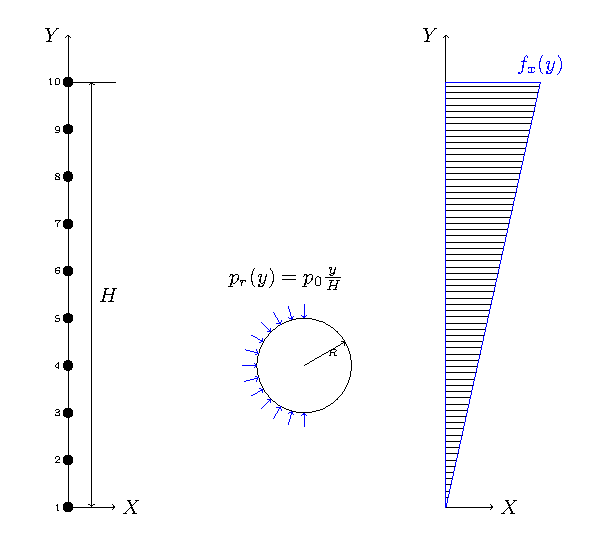
\includegraphics[width=0.8\textwidth]{example.pdf}
	\caption{测试算例示意图}
	\label{fig:example}
\end{figure}

\begin{table}[!htbp]
	\caption{测试算例输出节点集中力}
	\label{tab:example-force}
	\centering
	\begin{tabu} to 1.0\textwidth {X[c] X[2,c] X[2,c] X[2,c]}
		\toprule
		Node   & $F_X(\SI{}{N})$ & $F_Y(\SI{}{N})$ & $F_Z(\SI{}{N})$ \\
		\midrule
		1      & 5.527           & 0.000           & 0.000           \\
		2      & 22.526          & 0.000           & 0.000           \\
		3      & 44.996          & 0.000           & 0.000           \\
		4      & 66.994          & 0.000           & 0.001           \\
		5      & 88.994          & 0.000           & 0.001           \\
		6      & 110.991         & 0.000           & 0.000           \\
		7      & 132.990         & 0.000           & -0.002          \\
		8      & 154.990         & 0.000           & -0.001          \\
		9      & 176.987         & 0.000           & 0.002           \\
		10     & 93.992          & 0.000           & 0.002           \\
		$\sum$ & 898.987         & 0.000           & 0.003           \\
		\bottomrule
	\end{tabu}
\end{table}

\subsection{输电塔支撑构件的龙卷风荷载计算}

利用APDL命令流从输电塔结构有限元模型中提取相应于支撑构件的梁单元节点编号及坐标。
并通过下述方法计算支撑构件梁单元所受龙卷风荷载的方法。

首先,支撑构件梁单元某节点受到的风荷载可由下式计算\cite{savory2001modelling}:
\begin{equation}
	\bm{F_w} = \frac{1}{2} \rho_a C_d A |U| \bm{U}
\end{equation}
式中,$\rho_a$为空气密度,$C_d$为体型系数,本位取为$1.0$,$A$为该节点迎风投影面积,$\bm{U}$为风场在该节点处的风速矢量。
编制fluent UDF\todo{Add ref. for appendix}程序提取任意支撑节点$P(x, y, z)$在第\ref{sec:tornado-fsi}节模拟风场中的速度,算法如下:

\begin{enumerate}
	\item
	      首先判断出点$P$所在的计算流域网格控制体(可通过点$P$与某控制体各表面形心连线的向量与控制体表面法向量的关系判断点 是否属于该控制体);
	\item
	      提取该控制体的中心$C$点坐标$(x_c, y_c, z_c)$和$C$处的流场速度分量和速度梯度分量(将速度和各方向速度分量梯度矢量记为$\bm{U_C}$和$\bm{G_{CX}}$、$\bm{G_{CY}}$、$\bm{G_{CZ}}$);
	\item
	      利用下式计算点$P$处$X$方向速度分量为
	      \begin{equation}
	      	U_{PX} = U_{CX} + (\bm{OP}-\bm{OC})\cdot \bm{G_{CX}}
	      \end{equation}
	      $Y$和$Z$方向速度分量可类似计算。
\end{enumerate}


\section{输电塔龙卷风荷载计算的规范方法}\label{sec:static-code}

\subsection{龙卷风风场处理}
输电塔在龙卷风风场中的水平投影示意图如图\ref{fig:tower-tornado-cs}所示。
\begin{figure}[!htpb]
	\centering
	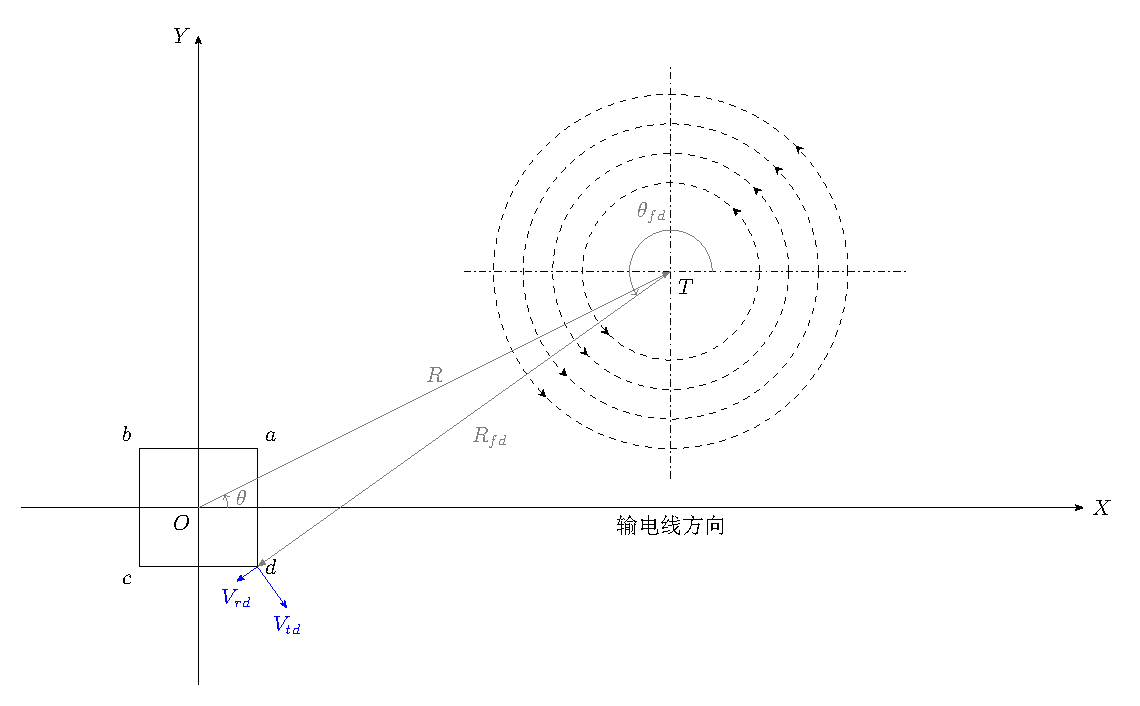
\includegraphics[width=\textwidth]{tower_tornado_cs.pdf}
	\caption{输电塔在龙卷风风场中的水平投影示意图}
	\label{fig:tower-tornado-cs}
\end{figure}
输电塔直角坐标系$\{O: XYZ\}$的建立方法见第\ref{sec:tower-fea}节。
$abcd$为输电塔处于同一水平剖面的节点。
下文主要展示推导$d$节点处龙卷风风速的方法,其余节点类似。
龙卷风中心在坐标系$\{O: XYZ\}$中的位置用极坐标$(R, \theta)$表示。
输电塔节点$d$相应于龙卷风核心的极坐标为$(R_{fd}, \theta_{fd})$,$d$节点受到的龙卷风切向、径向风速分别为$V_{td}$、$V_{rd}$,以及图\ref{fig:tower-tornado-cs}未明确表示的竖向风速$V_{ad}$。

\subsubsection{输电塔节点相应于龙卷风中心位置的极坐标}\label{sec:d-polor}
假设$d$节点在输电塔坐标系$\{O: XYZ\}$中的坐标为$(x_d, y_d, z_d)$,下文将推导节点$d$相应于龙卷风中心的极坐标$(R_{fd}, \theta_{fd})$。

龙卷风中心$T(R, \theta)$在输电塔坐标系$\{O: XYZ\}$中的直角坐标为$(R\cos\theta, R\sin\theta)$,则节点$d$相应于龙卷风中心$T$的向量为:
\begin{equation}
	\vv{Td} = \vv{Od} - \vv{OT} = (x_d - R\cos\theta, y_d - R\sin\theta) = R_{fd}(\cos\theta_{fd}, \sin\theta_{fd})
\end{equation}
式中,
\begin{equation}
	\begin{split}
		R_{fd} & = \sqrt{(x_d-R\cos\theta)^2+(y_d-R\sin\theta)^2} \\
		\theta_{fd} & = \arctan \frac{y_d - R\sin\theta}{x_d - R\cos\theta}
	\end{split}
\end{equation}

\subsubsection{龙卷风风场在直角坐标系下的分量}\label{sec:cs}
第\ref{sec:tornado}节模拟的龙卷风风场是定义在极坐标系下的,而施加风荷载采用直角坐标系下的风速分量较为简单,因此需要将龙卷风风场从极坐标系转化为直角坐标系。

输电塔节点$d$受到的龙卷风径向风速$V_{rd}$与$X$轴正方向的夹角为$\theta_{fd}$(图\ref{fig:tower-tornado-cs}),切向风速$V_{td}$与$X$轴正方向的夹角为$(\theta_{fd}+\pi/2)$,进行速度的分解如下:
\begin{equation}
	\begin{split}
		V_{xd} & = V_{rd} \cos\theta_{fd} + V_{td} \cos(\theta_{fd}+\pi/2) \\
		& = V_{rd} \cos\theta_{fd} - V_{td} \sin(\theta_{fd}) \\
		V_{yd} & = V_{rd} \sin\theta_{fd} + V_{td} \sin(\theta_{fd}+\pi/2) \\
		& = V_{rd} \sin\theta_{fd} + V_{td} \cos(\theta_{fd}) \\   
		V_{zd} & = V_{ad}  
	\end{split}
\end{equation}

有了上述准备工作,就可以计算输电塔上任意节点受到的龙卷风风速在直角坐标系下的分量了。

\subsubsection{龙卷风风场中任意节点处风速分量}
输电塔节点$d$相应于龙卷风中心的实际位置为$(R_{fd}, \theta_{fd})$(见第\ref{sec:d-polor}节),此节点对应于缩尺龙卷风风场$V_r(r,z)$、$V_t(r,z)$和$V_a(r,z)$(见第\ref{sec:tornado}节)中的位置为$(R_{md}, Z_{md})$,且
\begin{equation}
	\begin{split}
		R_{md} & = R_{fd} / L_s \\
		Z_{md} & = z_{fd} / L_s
	\end{split}
\end{equation}

在缩尺龙卷风风场中,由位置$(R_{md}, Z_{md})$可提取缩尺龙卷风风场径向、切向和竖向风速分量分别为$V_{rmd}$、$V_{tmd}$和$V_{amd}$。根据缩尺龙卷风速度相似比$V_s$可将其转化为足尺龙卷风风场中的速度分量:

\begin{equation}
	\begin{split}
		V_{rd} &= V_{rmd} \times V_s \\
		V_{td} &= V_{tmd} \times V_s \\
		V_{ad} &= V_{amd} \times V_s
	\end{split}
\end{equation}

最后根据第\ref{sec:cs}节的方法即可将输电塔节点$d$受到的极坐标系下的足尺龙卷风风速分量转化为直角坐标系下的风速分量。


\subsection{输电塔结构龙卷风风荷载计算}

\subsubsection{ASCE输电塔荷载规范风荷载计算方法}
ASCE主编的输电塔荷载规范 Guidelines for electrical transmission line structural loading\cite{wong2009guidelines}中输电塔风荷载计算公式为:
\begin{equation}
	F = \gamma_{\mathrm{w}} Q K_{\mathrm{z}} K_{\mathrm{zt}} \left( V_{50}\right)^2 G C_{\mathrm{f}} A
\end{equation}
其中:
\begin{description}[leftmargin=!,labelwidth=2em]
	\item[$F$] 顺风向风荷载
	\item[$\gamma_{\mathrm{w}}$] 考虑平均重现期的风荷载调整系数。平均重现期为$50$年时,$\gamma_{\mathrm{w}}=1.0$;平均重现期为$100$年时,$\gamma_{\mathrm{w}}=1.15$
	\item[$V_{50}$] 平均重现期为$50$年规定的风速基准值(基本风速)
	\item[$K_{\mathrm{z}}$] 风速压力暴露系数
	\item[$K_{\mathrm{zt}}$] 地形系数
	\item[$Q$] 将风速转化为速度压的常数,$Q=1/2 \rho_a=\SI{0.613}{kg/m^3}$
	\item[$G$] 阵风系数
	\item[$C_{\mathrm{f}}$] 风压系数
	\item[$A$] 迎风面构件的投影面积
\end{description}
各量中文翻译参考刘刚的论文\cite{liu2010wind}。

下面介绍ASCE规范中输电塔结构所受风荷载的风压系数$C_{\mathrm{f}}$的计算方法。

风压系数是密实度系数(solidity ratio)$\Phi$的函数,定义为:
\begin{equation}
	\Phi = \frac{A_\mathrm{m}}{A_\mathrm{o}}
\end{equation}
其中:
\begin{description}[leftmargin=!,labelwidth=2em]
	\item[$A_\mathrm{m}$] 迎风面构件的投影面积
	\item[$A_\mathrm{o}$] 塔架的轮廓面积
\end{description}
风压系数与密实度系数$\Phi$的关系表见图\ref{fig:force-coefficient}\cite{wong2009guidelines}
\begin{figure}[!htbp]
	\centering
	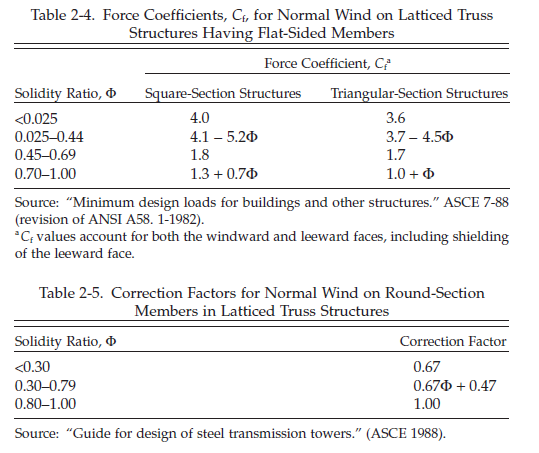
\includegraphics[width=\textwidth]{force_coefficient.png}
	\caption{风压系数}\label{fig:force-coefficient}
\end{figure}
方形截面的风压系数根据图\ref{fig:force-coefficient}中Table 2-4计算,圆形截面的风压系数根据Table 2-4的系数再乘上Table 2-5中的系数。

\subsubsection{中国架空输电线路设计规范风荷载计算方法}
中国《110~750kV架空输电线路设计规范》\cite{GB50545-2010}中杆塔风荷载的计算公式为:
\begin{equation}
	W_{\mathrm{s}} = W_{0} \cdot \mu_{\mathrm{z}} \cdot \mu_{\mathrm{s}} \cdot B_{2} \cdot A_{\mathrm{s}} \cdot \beta_{\mathrm{z}}
\end{equation}
\begin{equation}
	W_0 = V^2/1600
\end{equation}
式中:
\begin{description}[leftmargin=!,labelwidth=2em]
	\item[$W_{\mathrm{s}}$] 杆塔风荷载标准值(\SI{}{kN});
	\item[$W_{0}$] 基准风压标准值(\SI{}{kN/m^2});
	\item[$V$] 基准高度为\SI{10}{m}的风速(\SI{}{m/s});
	\item[$\mu_{\mathrm{z}}$] 风压高度变化系数
	\item[$\mu_{\mathrm{s}}$] 构件的体型系数,杆塔取$1.3(1+\eta)$,环形截面钢筋混凝土杆取$0.7$;
	\item[$B_{2}$] 杆塔构件覆冰风荷载增大系数,\SI{5}{mm}冰区取$1.1$,\SI{10}{mm}冰区取$1.2$,\SI{15}{mm}冰区取$1.6$,\SI{20}{mm}冰区取$1.8$,\SI{20}{mm}以上冰区取$2.0$~$2.5$;
	\item[$A_\mathrm{s}$] 迎风面构件的投影面积计算值(\SI{}{m^2});
	\item[$\eta$] 塔架背风面荷载降低系数,按表\ref{tab:eta}选用;
	\item[$\beta_\mathrm{z}$] 杆塔风荷载调整系数。
\end{description}

\begin{table}[!htbp]
	\caption{塔架背风面荷载降低系数$\eta$}
	\label{tab:eta}
	\centering
	\begin{tabu} to 1.0\textwidth {X[2,c] | X[c] X[c] X[c] X[c] X[c] X[c] }
		\toprule
		\diagbox{$b/a$}{$A_s/A$} & $\leq$ 0.1 & 0.2  & 0.3  & 0.4  & 0.5  & $>$ 0.6 \\
		\midrule
		$\leq$ 1                 & 1.0        & 0.85 & 0.66 & 0.50 & 0.33 & 0.15    \\
		2                        & 1.0        & 0.90 & 0.75 & 0.60 & 0.45 & 0.30    \\
		\bottomrule
	\end{tabu}
\end{table}

\subsubsection{中美规范计算输电塔龙卷风荷载参数取值}
美国输电塔荷载规范Guidelines for electrical transmission line structural loading\cite{wong2009guidelines}针对输电塔受到的龙卷风风荷载的建议为:考虑F2等级的龙卷风荷载,因为F2等级龙卷风发生的概率较高,且能够在经济投入允许的情况下加以设防;由于龙卷风风场速度为阵风风速,故风速压力暴露系数$K_\mathrm{z}$和阵风系数$G$取为$1.0$,即利用龙卷风风场的实际风速代入公式计算,不利用系数$K_\mathrm{z}$对其进行修正;由于龙卷风荷载是一种极端荷载情况,故考虑平均重现期的风荷载调整系数$\gamma_\mathrm{w}$取为$1.0$。

文献\cite{hamada2010finite}\cite{hamada2011behaviour}\cite{altalmas2014finite}等建议地形系数$K_\mathrm{zt}$取为$1.0$,因为龙卷风多发生在平坦开阔的平原。


参考美国输电塔荷载规范计算龙卷风荷载的参数取值建议,中国《110~750kV架空输电线路设计规范》的相关参数建议为:忽略覆冰荷载的影响,故杆塔构件覆冰风荷载增大系数取为$1.0$;忽略龙卷风的风振效应,将杆塔风荷载调整系数取为$1.0$。

\subsubsection{输电塔龙卷风荷载施加方法}
将输电塔分为多层,见图\ref{fig:tower-zone}所示,某具体层示意图见图\ref{fig:tower-zone-diagram}。
输电塔节点a,b,c和d上受到的龙卷风荷载的计算步骤如下:
\begin{figure}[!htbp]
	\centering
	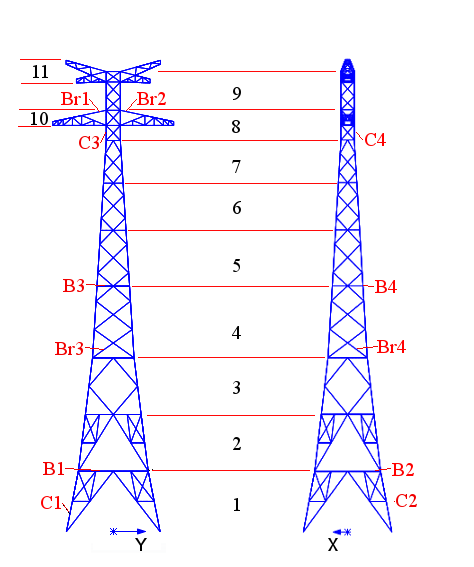
\includegraphics[width=0.6\textwidth]{tower_zone.png}
	\caption{输电塔分层示意图}\label{fig:tower-zone}
\end{figure}

\begin{figure}[!htbp]
	\centering
	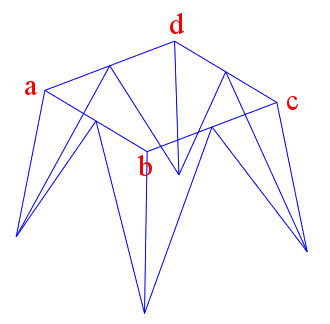
\includegraphics[width=0.6\textwidth]{tower_zone_diagram.png}
	\caption{输电塔典型层示意图}\label{fig:tower-zone-diagram}
\end{figure}

\begin{enumerate}
	\item 根据第\ref{sec:tornado}节计算输电塔节点a,b,c和d处龙卷风速度分量 $V_x$和$V_y$;
	\item 分别沿$X$和$Y$方向计算风速风量的均值$V_x'$和$V_y'$;
	\item 计算输电塔节点a,b,c和d处所在层龙卷风荷载,值得注意的是公式中各物理量采用SI单位制,即风速单位为\SI{}{m/s},风荷载单位为\SI{}{N}。
	      
	      根据美国ASCE规范,该层$X$和$Y$方向龙卷风荷载$F_{\mathrm{w}x}$和$F_{\mathrm{w}y}$为
	      \begin{equation}
	      	F_{\mathrm{w}x} = 0.613 (V_{x}')^2 C_{\mathrm{f}x} A_x
	      \end{equation}
	      \begin{equation}
	      	F_{\mathrm{w}y} = 0.613 (V_{y}')^2 C_{\mathrm{f}y} A_y
	      \end{equation}
	      其中,$A_x$和$A_y$分别为该层迎风面构件沿$X$和$Y$方向的投影面积。
	      风压系数由\ref{fig:force-coefficient}计算。
	      
	      根据中国规范,该层$X$和$Y$方向龙卷风荷载$F_{\mathrm{w}x}$和$F_{\mathrm{w}y}$为
	      \begin{equation}
	      	F_{\mathrm{w}x} = 0.625 (V_{x}')^2 \mu_{\mathrm{s}x} A_x 
	      \end{equation}
	      \begin{equation}
	      	F_{\mathrm{w}y} = 0.625 (V_{y}')^2 \mu_{\mathrm{s}y} A_y 
	      \end{equation}
	      体型系数$\mu_\mathrm{s} = 1.3(1+\eta)$,$\eta$由表\ref{tab:eta}计算。
	      
	      可知中美规范计算龙卷风荷载的公式的主要区别如下:中国将风速转化为速度压的系数为$\SI{0.625}{kg/m^3}$,美国为$1/2\rho_a=\SI{0.613}{kg/m^3}$,中国规范稍微偏保守;二者的主要差别为体型系数(风压系数)的计算:对于圆形截面输电塔,$\Phi<0.025$的层,美国规范的风压系数为$C_\mathrm{f}=4.0\times0.67=2.68$,中国规范为$\mu_\mathrm{s}=1.3(1+\eta)=1.3 \times(1+1.0)=2.6$,相差不大,美国规范偏保守。
	      
	\item 迎风面和背风面上风荷载分配
	      
	      中国规范根据塔架背风面荷载降低系数$\eta$对某层输电塔所受风荷载进行分配,即迎风面节点在$X$和$Y$方向所受风荷载分量分别为 $1/(1+\eta) F_{\mathrm{w}x}$ 和 $1/(1+\eta) F_{\mathrm{w}y}$;背风面节点在$X$和$Y$方向所受风荷载分量分别为 $\eta/(1+\eta) F_{\mathrm{w}x}$ 和 $\eta/(1+\eta) F_{\mathrm{w}y}$;
	      
	\item 迎(背)风面节点间风荷载分配
	      
	      迎(背)风面上的节点根据各节点的投影面积进行迎(背)风面上风荷载的分配。
	      
	      
\end{enumerate}


\subsection{索的悬链线理论及输电线作用于塔的荷载}

\subsubsection{索的悬链线理论基本假设}
索由高强钢丝集束而成,相对抗弯刚度很小,其受力特点可以认为是完全柔性。
在自重和张力作用下分析其线形和力学参数时,基本假设如下:
\begin{itemize}
	\item
	      索是理想柔性,既不能受压也不能受弯;
	\item
	      索的材料符合胡克定律;
	\item
	      索的横截面积在外荷载作用下的变化量十分微小,可忽略不计。
\end{itemize}

为了确定重力作用下索的线形,以弦左端点为原点、竖直向上为Y轴正方向建立右手直角坐标系。
则索受到的重力沿Y轴负向。
假设单位长度索的质量恒定,且不随张力变化。

\begin{figure}[!htbp]
	\centering
	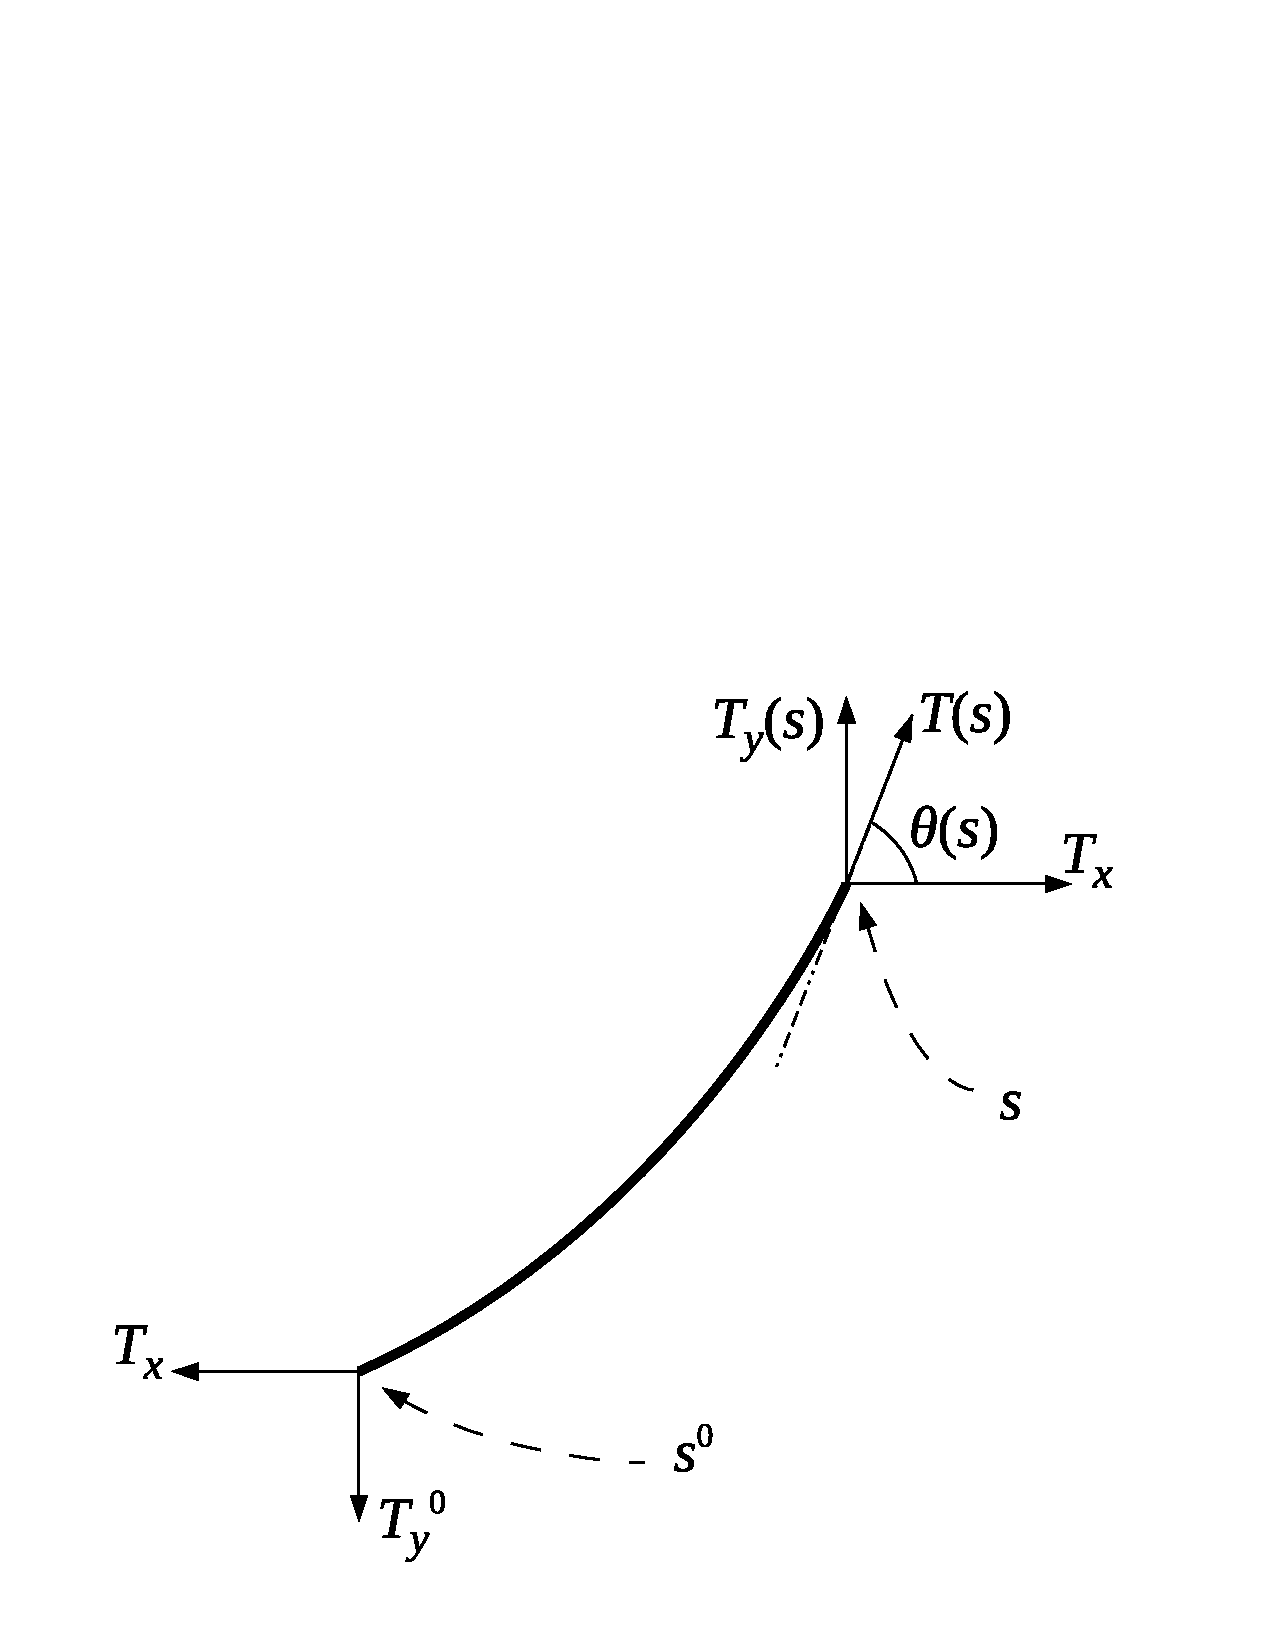
\includegraphics[width=0.6\textwidth]{catenary_diagram.pdf}
	\label{fig:catenary}
	\caption{索段计算示意图}
\end{figure}

\subsubsection{符号约定}
\begin{description}
	\item[$s$]
	从索左端点(坐标系原点)开始计算的索长度;
	\item[$\mu$]
	单位长度索的质量(假设是恒定的);
	\item[$T(s)$]
	索长度为$s$处的索张力(根据柔性索假设,张力沿索的切线方向);
	\item[$T_y(s)$]
	索长度为$s$处的索张力的$Y$向分量;
	\item[$T_x$]
	张力的$X$向分量(任取索段进行受力分析,由$X$向平衡方程可知$T_x$沿索长是均匀的);
	\item[$\theta(s)$]
	索切向量与$X$轴正向的夹角。
\end{description}

\subsubsection{自重作用下的单索线形求解}
索段竖向的平衡方程为:
\begin{gather}
	T_y(s) = g \int_{s^0}^{s} \mu \mathrm{d}s + T_y^0 \notag \\
	T_x \tan(\theta(s)) = g \mu \int_{s^0}^{s} \mathrm{d}s + T_y^0 \notag \\
	T_x \frac{\mathrm{d} y}{\mathrm{d} x} = g \mu \int_{s^0}^{s} \sqrt{1+\left(\frac{\mathrm{d} y}{\mathrm{d} x}\right)^2} \mathrm{d}x + T_y^0 \notag \\
	\frac{\mathrm{d}^2 y}{\mathrm{d} x^2} = \frac{g \mu}{T_x} \sqrt{1+\left(\frac{\mathrm{d} y}{\mathrm{d} x}\right)^2}
\end{gather}
此二阶微分方程的解析解为:
\begin{equation}
	y = \frac{T_x}{g \mu} \cosh \left( \frac{g \mu}{T_x} + c_1 \right)+c_2
\end{equation}
式中,$c_1$和$c_2$为由边界条件确定的积分常量。代入边界条件:$x=0,y=0;x=L,y=C$(见图\ref{fig:cat})。

\begin{figure}[!htpb]
	\centering
	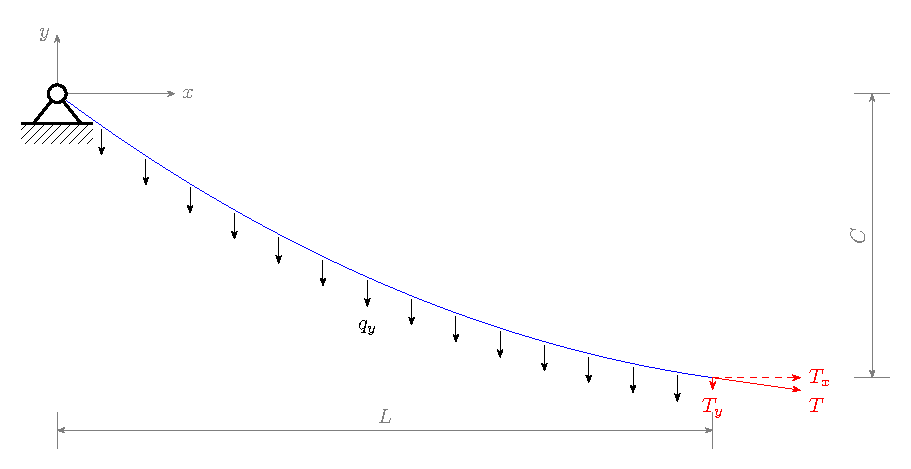
\includegraphics[width=0.8\textwidth]{cat.pdf}
	\caption{单缆尺寸及边界条件示意图}
	\label{fig:cat}
\end{figure}

\begin{equation}
	\left \{
	\begin{aligned}
		  & \beta = \frac{g \mu L}{2 T_x}                                \\
		  & c_1 = \sinh^{-1}\left(\frac{\beta C / L}{\sinh \beta}\right) \\
		  & c_2 = -\frac{T_x}{g \mu} \cosh(c_1)                          
	\end{aligned}
	\right.
\end{equation}

悬链线索的形状长度$S$和无应力长度$S_0$分别为:
\begin{equation}
	S = \frac{T_x}{g\mu}\left[\sinh\left(\frac{g \mu L}{T_x}+c_1\right)+\sinh(c_1)\right]
\end{equation}

\begin{equation}
	\begin{split}
		S_0 &= S-\Delta S \\
		&= S - \frac{T_x}{EA g \mu }\left[ \frac{1}{2} g \mu L + \frac{1}{8} T_x \left( e^{2(c_1+2\beta)} - e^{-2(c_1-2\beta)} -e^{2c_1} + e^{-2c_1} \right) \right]
	\end{split}
\end{equation}

\subsubsection{输电线施加在输电塔的荷载求解}

跨越塔之间输电线跨度为$L=\SI{1770}{m}$,右侧支座比左侧支座高度相同,即$C=\SI{0}{}$,跨中矢高$f=\SI{132.4}{m}$,单位长度质量$\mu=\SI{3219}{kg/km}$。
索的弹性模量$E=\SI{108070}{MPa}$,截面积$A=\SI{729}{mm^2}$。
假设在外荷载作用下两支座的间距及高差保持不变。
主要任务是利用上述悬链线理论计算输电线对输电塔施加的荷载。

主要思路:输电线在自重和张力作用下,其线形为悬链线,故可采用悬链线经典公式来进行求解。
采用直接建模的方式,单缆采用LINK1单元模拟,单元水平长度为\SI{1}{m}。
分析时,首先假定水平力大小,根据悬链线方程求解节点坐标,由此建立节点和单元,并分析单缆在自重作用下的内力和线形。
如果求解获得的水平力与假定水平力之间的误差较大或者单缆变形较大,则返回重新计算,直至满足误差要求。计算框图如图\ref{fig:flow-chart}所示。

\begin{figure}[!htpb]
	\centering
	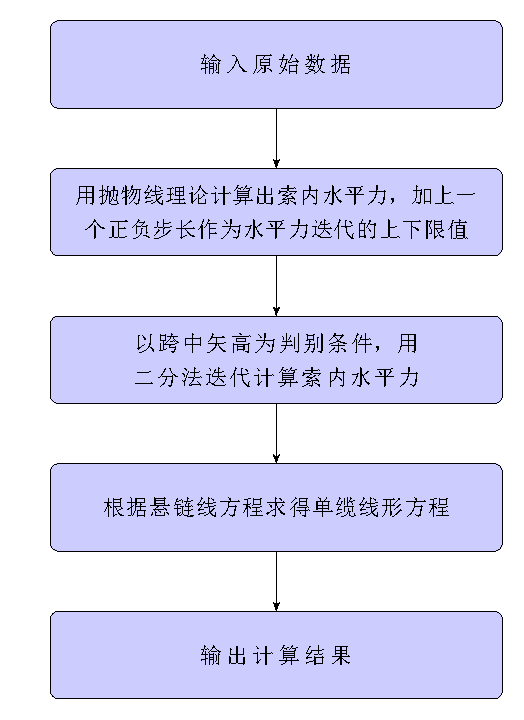
\includegraphics[width=0.4\textwidth]{flow_chart.pdf}
	\caption{单缆线形和力学参数计算框图}
	\label{fig:flow-chart}
\end{figure}

计算的APDL和MATLAB程序见附录\ref{apen:cat}。
单缆最大位移为\SI{12.7}{mm},相比于跨径$L=\SI{1770}{m}$该变形已足够小,认为已满足精度要求。

对于跨越塔和锚塔之间的输电线对跨越塔的荷载计算采用相同的方法,在此不一一列举。

跨越塔受到的两侧输电线传来的张力的示意图见图\ref{fig:line-force}所示。

\begin{figure}[!htbp]
	\centering
	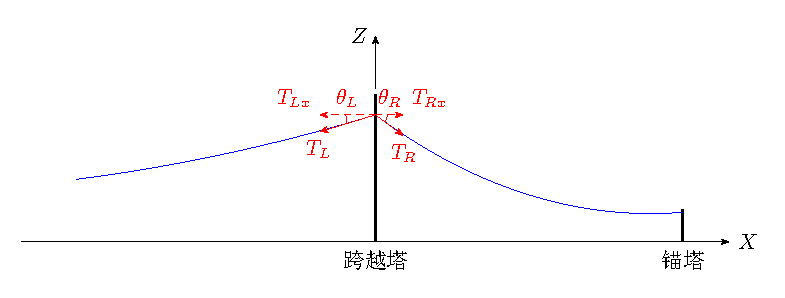
\includegraphics[width=0.8\textwidth]{line_force}
	\caption{跨越塔受到输电线的张力示意图}
	\label{fig:line-force}
\end{figure}

经过附录\ref{apen:cat}程序的计算,图\ref{fig:line-force}中各量为:
\begin{equation}
	\begin{split}
		T_{Lx} & = \SI{93.31}{kN},\quad \theta_L  = \ang{16.89} \\
		T_{Rx} & = \SI{21.33}{kN},\quad \theta_L  = \ang{36.70}
	\end{split}
\end{equation}


\section{FSI方法与规范方法的对比}

为了考虑最不利工况,将龙卷风核心距离输电塔中心的径向距离设置为龙卷风核心半径$R_T=r_{c,\mathrm{mat}}=\SI{120}{m}$,
$\theta_T$分别取\SI{0}{\degree}、\SI{45}{\degree}和\SI{90}{\degree}。
分别根据单向流固耦合方法(FSI方法)和规范方法计算并施加龙卷风荷载,进行输电塔结构的静态响应分析。
输电塔结构最大轴向压力和位移响应随袭击角$\theta_T$的变化见图\ref{fig:fx-vs-theta}和图\ref{fig:disp-vs-theta}所示。
代表性构件(见图\ref{fig:tower-zone}所示)的轴向力取得极值的工况见表\ref{tab:axial-force}所示。

\begin{figure}[!htbp]
	\centering
	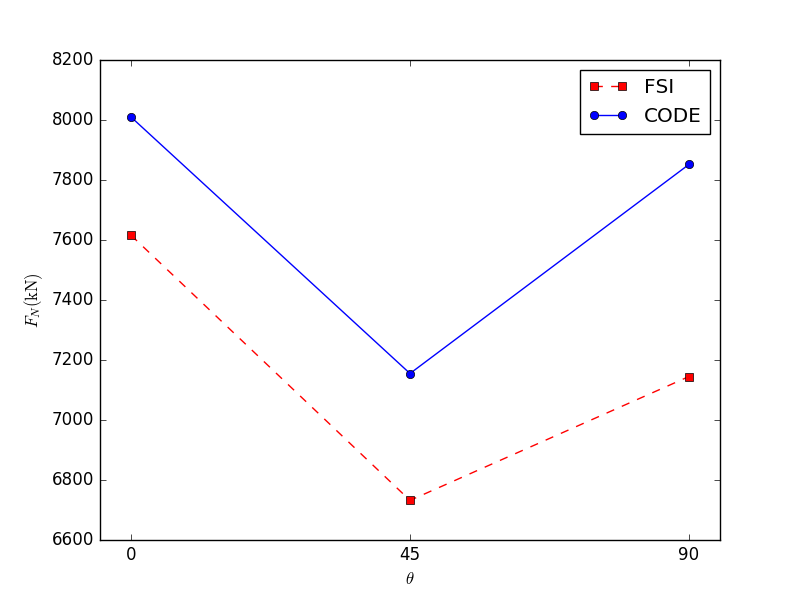
\includegraphics[width=0.8\textwidth]{Fx_vs_theta.png}
	\caption{输电塔构件最大轴向压力随袭击角的变化}
	\label{fig:fx-vs-theta}
\end{figure}

\begin{figure}[!htbp]
	\centering
	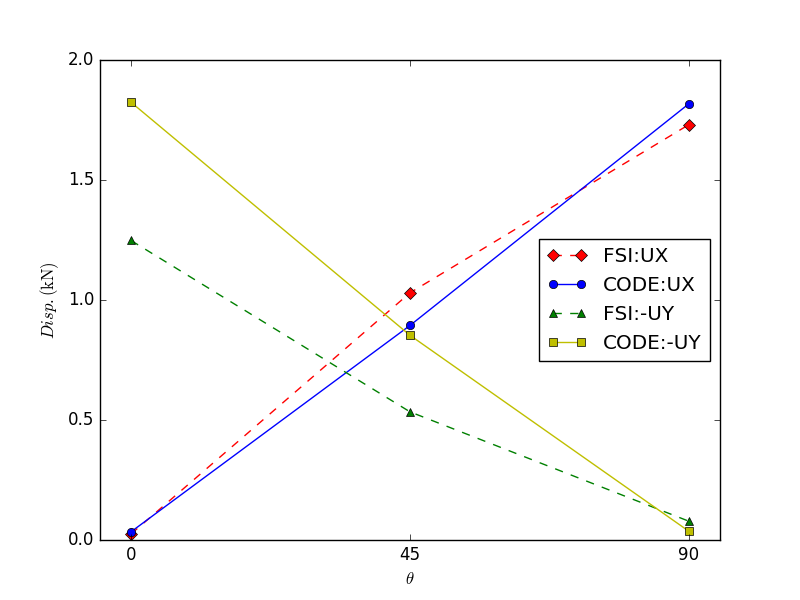
\includegraphics[width=0.8\textwidth]{Disp_vs_theta.png}
	\caption{输电塔构件最大位移分量随袭击角的变化}
	\label{fig:disp-vs-theta}
\end{figure}

\begin{table}[!htbp]
	\caption{输电塔代表构件的轴向力}
	\label{tab:axial-force}
	\centering
	\begin{tabu} to 1.0\textwidth {X[c] X[c] X[2,c] X[c] X[2,c] X[c]}
		\toprule
		\multicolumn{2}{c}{构件} & \multicolumn{2}{c}{单向流固耦合} & \multicolumn{2}{c}{规范方法} \\
		编号 & 类型 & 轴向内力(\SI{}{kN}) & 角度(\SI{}{\degree}) & 轴向内力(\SI{}{kN}) & 角度(\SI{}{\degree}) \\
		\midrule
		C1	& 柱	& -6485	& 90 & 	-7803	& 90  \\
        C2	& 柱	& 7739	& 0	 &   8154	& 0  \\
        C3	& 柱	& -4958	& 90 &	-5024	& 90  \\
        C4	& 柱	& 5700	& 0	 &   5762	& 0  \\
        B1	& 梁	& 328	& 90 &	488	    & 90  \\
        B2	& 梁	& -274	& 0	 &  -316	& 0  \\
        B3	& 梁	& 87	& 0	 &   120	& 90  \\
        B4	& 梁	& -123	& 90 &	-130	& 90  \\
        Br1	& 支撑	& -27	& 45 &	-51	    & 45  \\
        Br2	& 支撑	& -42	& 45 &	-71	    & 45  \\
        Br3	& 支撑	& 318	& 90 &	588	    & 90  \\
        Br4	& 支撑	& -268	& 0	 &  -371	& 0  \\
		\bottomrule
	\end{tabu}
\end{table}

采用单向流固耦合和规范方法计算得到的输电塔结构响应整体上吻合较好,表
\ref{tab:axial-force}所列构件中,二者最大误差不超过$50\%$。

\section{本章小结}
本章分别利用单向流固耦合方法和规范方法计算并施加龙卷风荷载到输电塔结构有限元模型上,并在0度,45度和90度袭击角工况下比较了两种方法计算得到的结构响应。

首先根据\SI{500}{kV}南京三江口大跨越工程中跨越塔建立有限元模型,并进行模态分析提取结构固有频率,与文献进行对比以验证结构有限元模型的正确性。

然后在忽略龙卷风平移运动的影响下,选定龙卷风核心相应于输电塔结构中心的位置,进行静力弹塑性分析。
输电塔受到的龙卷风荷载分别通过单向流固耦合方法和规范中风荷载公式计算。

单向流固耦合方法直接在足尺龙卷风风场中建立结构主体梁柱框架的刚性模型,通过CFD计算得到刚性模型表面受到的龙卷风风压,并编程将风压转化为输电塔梁单元模型的节点集中力;
对于支撑等迎风效应(截面尺寸)较小的构件,直接提取风场中相应于支撑构件节点处的风速,并利用阻力系数将风速转化为节点荷载。
将这两部分荷载均施加到结构有限元模型上,进行静力弹塑性分析,进而提取结构响应。

规范方法先对足尺龙卷风数值风场进行处理,转化成切向、径向风速在不同高度处随径向距离的分布;
并推导公式计算输电塔任意节点受到龙卷风在整体直角坐标系下风速分量;
然后简要比较了美国Guidelines for electrical transmission line structural loading规范和中国《110 ~ 750kV 架空输电线路设计规范》中风荷载计算公式,并将输电塔结构分成多层,分层施加龙卷风荷载。

输电塔还受到输电线传来的荷载,本章利用索的悬链线理论进行计算。

最后考虑最不利工况,将龙卷风核心与输电塔中心的距离设置为龙卷风核心半径$R_T=r_{c,max}=\SI{120}{m}$,袭击角分别取为$\SI{0}{\degree}$、$\SI{45}{\degree}$和$\SI{90}{\degree}$。
分别利用单向流固耦合方法和规范方法计算龙卷风荷载,分析比较结构的最大轴向力和位移响应。
发现采用单向流固耦合和规范方法计算得到的输电塔结构响应整体上吻合较好,按两种方法计算的结构轴向力和位移响应随袭击角的变化趋势相似,且轴向力误差不超过$20%$,位移响应误差不超过$30\%$,可以互相验证。
\SI{45}{\degree}工况下结构在$X$和$Y$方向均发生变形,会出现整体的扭转变形。
两种方法计算的代表性构件的轴力,梁柱等关键构件轴力误差较小,支撑等次要构件轴向力响应误差较大,但误差不超过$50\%$。

